\documentclass[twocolumn,a4paper,dvipdfmx]{ieicejsp}
\usepackage[T1]{fontenc}
\usepackage{lmodern}
\usepackage{textcomp}
\usepackage{latexsym}
\usepackage{float}
\usepackage{graphicx}
\usepackage{amsmath, amssymb}
\usepackage{bm}
\usepackage{caption}
\usepackage{booktabs}
\usepackage{multirow}
\usepackage{url}
\usepackage{xcolor}
\usepackage{tikz}
\usetikzlibrary{positioning, arrows.meta}
\captionsetup{font=small}
\renewcommand{\dbltopfraction}{0.9}
\renewcommand{\topfraction}{0.9}
\renewcommand{\textfraction}{0.1}
\setcounter{dbltopnumber}{2}
\newcommand{\rev}[1]{{\color{red}#1}}
\DeclareMathOperator*{\argmax}{arg\,max}

\title{
    {{\bf {OWLv2，Alpha-CLIPと語彙の木を用いた\\再学習を必要としない粒度可変の物体アノテーション}}
    {\normalsize \\ {Training-Free Adjustable-Granularity Object Annotation with OWLv2, Alpha-CLIP, and a Vocabulary Tree}}}
}
\author{
    著者名 \\ Author Name
}
\affliate{%
    所属機関名 \\
    Affiliation \\
}

\begin{document}
\maketitle

\begin{abstract}
物体領域の検出とカテゴリのアノテーションを分離し，\rev{WordNetとVisual Genome（VG）を組み合わせた語彙の木}をたどってカテゴリの粒度を変更する，再学習を必要としない物体アノテーションのモデルを示す．
本モデルは，検出器にOWLv2のクラス非依存の物体らしさ，分類器に注目領域をマスクで与えるAlpha-CLIPを用い，\rev{語彙の木の全ての語}の確率を語彙の木の部分木ごとに合計して，確信度に応じた深さの語を出力する．
検出器と分類器をそれぞれ置き換えた場合と比較し，各部品を選ぶ理由を示す．
COCO 2017 Validationの500枚による評価では，OWLv2は1枚あたり50個のボックスでCOCOの物体の87.5\%を囲み，DETRの73.8\%とYOLO11xの70.2\%を上回った．
同じ画像のLVISの注釈によるCOCO外の物体の再現率は，OWLv2の73.4\%に対してYOLO11xは10.0\%，DETRは12.4\%であり，COCOで学習した検出器はCOCO外の物体をほとんど囲めなかった．
一方，COCOの80クラスによるF値は，検出器をYOLO11xのボックスに替えた構成が0.535，DETRが0.486，OWLv2が0.411であり，COCOの物体に限ればCOCOで学習した検出器のボックスが有利であった．
分類器は，いずれの検出器でもAlpha-CLIPのF値がCLIPより0.03〜0.05高く，COCOのクラスより細かい語を正しく出力した割合もCLIPの約2倍であった．
GTのボックスに対する命名では，部分木の確率の合計により，COCOのクラスのみで命名する場合と比べて階層的F値が0.266から0.639に向上した．
\end{abstract}

\noindent
{\bf キーワード：}物体アノテーション，粒度可変アノテーション，WordNet，Visual Genome，OWLv2，Alpha-CLIP，YOLO，DETR，オープンボキャブラリ

\section{はじめに}
画像データセットに対する物体アノテーションは，物体が画像のどこに存在するかという物体領域の判断と，その物体が何であるかというカテゴリの判断から構成される．
YOLO\cite{ref_YOLO}やDETR\cite{ref_DETR}に代表される物体検出モデルは，両者を学習時に定めた固定のクラス集合に対して行うため，COCO\cite{ref_COCO}の80クラスで学習したモデルは，80クラスより細かい語や80クラスの外の語を出力できない．
新しいクラスを扱うには，そのクラスの注釈を集めて再学習する必要がある．

著者らの前稿\cite{ref_prev,ref_prevVG}では，物体領域の検出とカテゴリのアノテーションを分離し，検出した領域に視覚言語モデル（Vision-Language Model，VLM）のゼロショット分類を適用して，WordNet\cite{ref_WordNet}の下位語をたどることで再学習なしにカテゴリの粒度を変更する手法を検討した．
前稿の構成は，DETRのボックスの切り抜き画像にCLIP\cite{ref_CLIP}を適用するものであった．
本稿では，検出器をOWLv2\cite{ref_OWLv2}のクラス非依存の物体らしさに，分類器を注目領域をマスクで与えるAlpha-CLIP\cite{ref_AlphaCLIP}に置き換え，前稿\cite{ref_prevVG}の\rev{WordNetとVisual Genome（VG）\cite{ref_VG}を組み合わせた語彙の木}で粒度を決めるモデルを示す．

このモデルでは，検出器がアノテーションできる物体の範囲を決め，分類器と語彙の木が出力する語の正しさと細かさを決める．
COCOで学習したYOLOやDETRはCOCOの物体を少ないボックスで正確に囲むが，COCO外の物体の領域を出力するかは明らかでない．
OWLv2の物体らしさは学習時のクラスに依存しないが，ボックスの数が多くなる．
また，CLIPに切り抜き画像を入力すると周囲の文脈が失われ，Alpha-CLIPで領域を指定する場合との差は明らかでない．
そこで本稿では，モデルの各部品を置き換えた構成と比較し，部品を選ぶ理由を実験により示す．

本稿の貢献は以下の3点である．
第一に，提案手法の検出器をOWLv2，YOLO11x，DETRの3つで比較し，COCOの物体の再現率，COCO外の物体の再現率，検出から命名までのF値を示す．
これにより，COCOの物体に限ればYOLO11xとDETRのボックスが有利である一方，COCO外の物体を囲めるのはOWLv2のみであることを示し，OWLv2を選ぶ理由を明らかにする．
第二に，分類器をCLIPとAlpha-CLIPで比較し，いずれの検出器でもAlpha-CLIPのF値と，COCOのクラスより細かい語を正しく出力する割合が高いことを示す．
第三に，\rev{WordNet$ \cap $VGの木（\ref{sec_vocab}節）}の部分木ごとに語の確率を合計して出力の深さを決める命名が，WordNetの下位語を1段ずつたどる命名より細かい粒度の評価を高めることを，GTのボックスで示す．
なお，検出したボックスのうちどれを残すかを決める棄却の判定について，本稿では単純な規則を用い，その設計は今後の課題とする．

\section{関連研究}
\subsection{物体検出とオープンボキャブラリ}
YOLO\cite{ref_YOLO}とDETR\cite{ref_DETR}は，学習時に定めたクラス集合を前提とする物体検出モデルである．
CLIP\cite{ref_CLIP}は，画像とテキストの対の対照学習により，自然言語で指定した概念へのゼロショットの転移を可能にした．
OWL-ViT\cite{ref_OWLViT}とOWLv2\cite{ref_OWLv2}は，CLIPの画像エンコーダの各パッチからボックスを予測し，テキストで指定したカテゴリの物体を検出する．
OWLv2はクエリとは別に，クラス非依存の物体らしさのスコアも出力する．
Alpha-CLIP\cite{ref_AlphaCLIP}は，CLIPの画像エンコーダのパッチ埋め込みに注目領域を表すαチャネルの畳み込みを加え，画像全体の文脈を保ったまま指定した領域の特徴を求める．

\subsection{語彙と意味の階層}
VG\cite{ref_VG}は，10万枚を超える画像に物体を密に注釈し，物体の名前をWordNetのSynsetに正規化している．
前稿\cite{ref_prevVG}では，VGの注釈のSynsetの出現頻度から語彙を構成し，人手で定めた最上位の枠とWordNetの上下関係で木を作った．
さらに，全ての語の確率を部分木ごとに合計し，合計が閾値を超える最も深いノードを出力することで，COCO外の物体の命名を改善した．
下位クラスで分類してから親のクラスへ写像するCHiLS\cite{ref_CHiLS}も，具体的な語の確率を集約して粗い判断に用いる点で共通する．
階層のあるカテゴリの評価には，正解と出力の上位語の集合の重なりに基づく階層的適合率と階層的再現率\cite{ref_hier}を用いる．
本稿は，前稿の語彙の木による命名を，クラス非依存の検出器と領域を指定する分類器と組み合わせ，検出器と分類器の選択が命名の粒度と正しさに与える影響を調べる点が異なる．

\section{提案手法}
\subsection{全体の流れ}
図\ref{fig_pipeline}に提案するモデルの流れを示す．
画像$ {\mathbf X} $からOWLv2の物体らしさでボックスを1回の推論で検出し，各ボックスの領域の特徴をAlpha-CLIPで求める．
次に，\rev{WordNet$ \cap $VGの木}の全ての語の確率を求め，部分木ごとに確率を合計する．
部分木の確率の合計から，ボックスを残すかと深さ0のラベル（COCOのクラス）を決め，確信度に応じた深さの語を出力する．
出力した語から根までの経路を切り詰めることで，任意の粗さの語も得られる．
いずれの段階も追加の学習を行わない．

\begin{figure}[t]
\centering
\resizebox{\linewidth}{!}{%
\begin{tikzpicture}[node distance=2.5mm, every node/.style={font=\scriptsize}, box/.style={draw, rounded corners=1pt, align=center, minimum height=6mm, inner sep=1.5pt}, >=Stealth]
\node[box] (img) {画像\\$ {\mathbf X} $};
\node[box, right=of img] (owl) {OWLv2\\物体らしさ$ o_k $};
\node[box, right=of owl] (alpha) {Alpha-CLIP\\領域の特徴};
\node[box, right=of alpha] (prob) {\rev{WordNet$ \cap $VG}\\の確率$ p_w $};
\node[box, below=4mm of prob] (mass) {部分木の\\合計$ m_u $};
\node[box, left=of mass] (rej) {ラベル$ c_k $\\ボックスの選択};
\node[box, left=of rej, fill=yellow!20] (dedup) {出力の深さ\\$ u^{*}_k $};
\node[box, left=of dedup] (out) {出力\\（粒度可変）};
\draw[->] (img) -- (owl); \draw[->] (owl) -- (alpha); \draw[->] (alpha) -- (prob); \draw[->] (prob) -- (mass);
\draw[->] (mass) -- (rej); \draw[->] (rej) -- (dedup); \draw[->] (dedup) -- (out);
\end{tikzpicture}}
\caption{提案するモデルの流れ．網掛けは粒度を決める段階である．}
\label{fig_pipeline}
\end{figure}

\subsection{検出と領域の特徴}
OWLv2の物体らしさのスコア$ o_k $の降順に，クラス非依存のNMS（IoU 0.5）を適用したボックス$ {\mathbf b}_k $を用いる．
1画像あたりの平均のボックス数$ B $が所定の値になるよう，検証用の画像のスコアから物体らしさの閾値を定める．
検出器の比較では，OWLv2をCOCOで学習したYOLO11x\cite{ref_YOLO11}またはDETR\cite{ref_DETR}に置き換える．
この場合も各検出器が出力するクラスは用いず，ボックスと検出スコアのみを用い，検出スコアを$ o_k $とする．
したがって，検出器を置き換えても，命名と粒度の変更は\rev{WordNet$ \cap $VGの木}で行い，再学習は必要としない．

各ボックスの領域の特徴は，Alpha-CLIPの画像エンコーダで求める．
入力には，ボックスに合わせて切り抜いた画像を長辺に合わせて黒で埋めた正方形（以下，crop）と，ボックスの長辺の1.5倍の正方形の窓（以下，context）の2通りを用いる．
αチャネルには，ボックスの内側を1，外側を0とするマスクを与える．
分類器の比較では，Alpha-CLIPをCLIP（ViT-B/32）に置き換え，cropの画像をαチャネルなしで入力する．
語$ w $の確率は，CLIPと同じく

\begin{equation}
    p_w({\mathbf b}_k) = \frac{\exp\bigl(t \cos(g_I({\mathbf b}_k), g_T(w))\bigr)}{\sum_{w' \in {\mathbb W}} \exp\bigl(t \cos(g_I({\mathbf b}_k), g_T(w'))\bigr)}
    \label{eq_prob}
\end{equation}

\noindent
とする．
ここで，$ g_I $と$ g_T $は画像と文章のエンコーダ，$ g_T(w) $はプロンプト``a photo of a \{$w$\}''の特徴，$ t $は学習済みの温度，$ {\mathbb W} $は語彙である．

\subsection{語彙の木と部分木の確率の合計}\label{sec_vocab}
前稿\cite{ref_prevVG}と同じく，VGの物体の注釈のSynset $ s $の出現回数を$ n(s) $とし，語彙を

\begin{equation}
    {\mathbb V} = \{ s \mid n(s) \geq 10,\ d(s) \geq 5 \} \cup {\mathbb C}
    \label{eq_vocab}
\end{equation}

\noindent
とする．
ここで，$ d(s) $はWordNetの根からの最短の深さ，$ {\mathbb C} $はCOCOの80クラスのSynsetの集合である．
プロンプトには，各Synsetに対してVGの注釈者が最も多く用いた名前を用いる．
語彙の語は，上位語をたどって至る段数が最小の最上位の枠（$ J = 40 $）に割り当て，同じ枠の中で上位語をたどって最初に出会う語彙の語を親とする．
親が無い語は枠を親とし，どの枠にも含まれない語は仮想的な枠にまとめる．
\rev{語はVGに現れるWordNetのSynset，親子はWordNetの上下関係であるため，これをWordNet$ \cap $VGの木と呼ぶ．}

ノード$ u $の部分木に含まれる語の集合を$ {\mathbb D}(u) $とし，部分木の確率の合計を

\begin{equation}
    m_u({\mathbf b}_k) = \sum_{w \in {\mathbb D}(u)} p_w({\mathbf b}_k)
    \label{eq_mass}
\end{equation}

\noindent
とする．
深さ0のラベルの決定には$ T = 1 $（式(\ref{eq_prob})のまま）の確率を用いる．
COCOの80クラスのノードの部分木には，そのクラスの下位語の語彙の語が含まれる．
例えばpersonの部分木には，man，woman，player，skierなど136語が含まれる．

\subsection{深さ0のラベルと残すボックス}
各ボックスの深さ0のラベル$ c_k $と，ボックスを残すかを決めるスコア$ r_k $を，COCOのクラスのノードの部分木の確率の合計を用いて

\begin{equation}
    c_k = \argmax_{c \in {\mathbb C}} m_c({\mathbf b}_k), \quad r_k = m_{c_k}({\mathbf b}_k) \, o_k
    \label{eq_score}
\end{equation}

\noindent
とする．
VLMが人物の領域で持ち物の名前の確率を最大にしても，人物の多くの下位語の確率がpersonの部分木に集まるため，人物のボックスにpersonのラベルを付けることができる．
$ r_k $の降順に，同じラベルのボックスとIoUが0.5以上のボックスと，面積の80\%以上が同じラベルのボックスに含まれるボックスを除き，$ r_k \geq \theta $のボックスを残す．
本稿ではこの規則を全ての構成に共通に用い，残すボックスを決める規則の設計は今後の課題とする．

\subsection{部分木の確率の合計による粒度の変更}
残したボックスの出力する語は，前稿\cite{ref_prevVG}と同じく，温度$ T $の確率から求めた$ m_u $が閾値$ \tau $以上のノードのうち，深さが最大（同じ深さなら$ m_u $が最大）のノード

\begin{equation}
    u^{*}_k = \argmax_{u: m_u \geq \tau} \bigl(\mathrm{depth}(u), m_u({\mathbf b}_k)\bigr)
    \label{eq_output}
\end{equation}

\noindent
とする．
確信度が低い場合はより粗いノードが選ばれ，出力したノードから根までの経路を切り詰めることで，粗い粒度のカテゴリも得られる．
例えば，テニス選手の領域でtennis playerの確率が$ \tau $を超えればtennis playerを出力し，下位語の確率が分散してどの語も$ \tau $を超えない場合でも，部分木の合計が大きいpersonを出力する．
このように，語彙の木の構造と確率の合計のみで粒度を決めるため，語彙や木を差し替えても再学習は必要としない．

\section{実験}
\subsection{共通設定}
評価にはCOCO 2017 Validationを用いた．
前稿\cite{ref_prev}と同じく，seed 42で選んだ500枚を検証用，別の500枚をテスト用とした．
テスト用の画像のGTの物体は3458件（人物1090件，人物以外2368件）である．
閾値などの条件は全て検証用の画像で選び，テスト用の画像の結果を報告する．
COCO外の物体の評価には，テスト用の画像のうちLVIS v1\cite{ref_LVIS}の注釈がある474枚を用い，Synsetが COCOのクラスのSynsetの上位語，下位語，自身のいずれでもない2687件をCOCO外の物体とした．
VGの語彙にはVG v1.2の108077枚の物体の注釈を用い，COCO 2017 Validationと重複する2186枚を集計から除いた．
式(\ref{eq_vocab})の語彙は3263語（COCOの80クラスを加えて3293語），木は枠を含めて3315ノードである．
最上位の枠は前稿に一覧が無いため，clothing，furniture，animal，light，natural objectなどの40個を定めた．

検出器には，OWLv2（ViT-B/16，ensemble）\cite{ref_OWLv2}の物体らしさ（$ B = 20, 50 $），YOLO11x\cite{ref_YOLO11}（検出スコア0.25以上），DETR（ResNet-50，検出スコア0.5以上）\cite{ref_DETR}を用いた．
分類器には，Alpha-CLIP（ViT-B/16）\cite{ref_AlphaCLIP}とCLIP（ViT-B/32）\cite{ref_CLIP}を用いた．
参照として，前稿の構成（以下，Old）であるDETRのボックスの切り抜き画像にCLIPを適用し，COCOの80クラスの最大の確信度でボックスを残すものと，COCOで学習したYOLO11xが出力するクラスをそのまま用いるもの（以下，YOLO11x単体）を評価した．
YOLO11x単体以外は，いずれもCOCOのクラスの注釈を命名に用いない．
GPUにはNVIDIA GeForce RTX 4070 Tiを用い，いずれのモデルも再学習は行わない．

\begin{table}[t]
\centering
\caption{本稿の表で用いる記号と評価指標．}
\label{tab_metrics}
\setlength{\tabcolsep}{3pt}
\begin{tabular}{lp{0.68\linewidth}}
\toprule
記号 & 説明 \\
\midrule
$ B $ & OWLv2の1枚あたりの平均ボックス数（閾値を検証用の画像で決める） \\
$ N $ & 1枚あたりのボックス数（式(\ref{eq_score})の規則の後は残した数） \\
$ R_{\rm all} $ & 検出の再現率：クラスを問わずIoU 0.5以上のボックスがあるGTの割合 \\
$ R_{\rm per} $，$ R_{\rm oth} $ & $ R_{\rm all} $の人物のGT，人物以外のGTに限った値 \\
$ R_{\rm N} $ & COCO外の物体の再現率：LVISのCOCO外の物体を囲んだ割合 \\
$ E $ & どのGTともIoU 0.5以上で重ならないボックスの割合 \\
$ t $ & 1枚あたりの検出の時間（秒） \\
Top-1 & 対応したボックスのうち，ラベルがGTのクラスと一致した割合 \\
$ P $，$ R $，$ F $ & 適合率，再現率，F値：ラベルも一致した組を正解とする（COCOの80クラス） \\
$ hP $，$ hR $，$ hF $ & 細かい正解に対する階層的適合率，階層的再現率，階層的F値（式(\ref{eq_hier})） \\
$ \tau $，$ T $ & 出力の深さを決める確率の閾値と温度（式(\ref{eq_output})） \\
$ R_{\rm p} $ & 人物の再現率：人物のGTのうち，対応したボックスを残した割合 \\
Acc & 命名の正解率：細かい正解と一致，それより細かい，または正しい上位語を出力した割合 \\
Fine & 正しくCOCOのクラスより細かい語を出力した割合 \\
\bottomrule
\end{tabular}
\end{table}

評価指標を表\ref{tab_metrics}に示す．
COCOの80クラスによる指標では，スコアの降順に，IoUが0.5以上のGTと1対1に対応付け，Top-1，$ P $，$ R $，$ F $を求めた．
細かい粒度の指標では，COCOのキャプションの名詞をspaCyで取り出してWordNetの第1語義に変換し，GTのクラスのSynsetの真の下位語になる語を，その画像の同じクラスのインスタンスの細かい正解とした（例：person→man，woman，tennis player）．
細かい正解を持つインスタンスはテスト用の画像で912件であり，85\%が人物である．
前稿\cite{ref_prevVG}と同じく，出力$ u $と細かい正解$ g $について，Synset自身と深さ4以上の上位語の集合$ {\mathbb P}_k $，$ {\mathbb G}_k $を求め，

\begin{equation}
    hP = \frac{\sum_k |{\mathbb P}_k \cap {\mathbb G}_k|}{\sum_k |{\mathbb P}_k|}, \quad hR = \frac{\sum_k |{\mathbb P}_k \cap {\mathbb G}_k|}{\sum_k |{\mathbb G}_k|}
    \label{eq_hier}
\end{equation}

\noindent
とし，その調和平均を$ hF $とした．
ただし，person.n.01の深さは3であるため，COCOの80クラスのSynsetは深さによらず集合に含めた．
未検出または残さなかったインスタンスは$ {\mathbb P}_k = \emptyset $とする．
差の検定には，画像単位の対応のあるブートストラップ（1000回）を用いた．
式(\ref{eq_score})の$ \theta $は検証用の画像の$ F $で，式(\ref{eq_output})の$ T $と$ \tau $は検証用の画像の$ hF $で選んだ（Alpha-CLIPは$ T = 1 $，$ \tau = 0.05 $，CLIPは$ T = 1.5 $，$ \tau = 0.1 $）．

\subsection{検出器の比較}
\begin{table}[t]
\centering
\caption{検出器のみの比較（テスト用の画像）．$ R_{\rm N} $はLVISの注釈がある474枚のCOCO外の物体2687件に対する値，その他はCOCOのGT 3458件に対する値である．記号は表\ref{tab_metrics}による（$ N $：ボックス数，$ R_{\rm all} $：再現率，$ R_{\rm per} $：人物の再現率，$ R_{\rm oth} $：人物以外の再現率，$ E $：GTに当たらない割合，$ R_{\rm N} $：COCO外の物体の再現率，$ t $：時間）．}
\label{tab_detector}
\setlength{\tabcolsep}{2.5pt}
\resizebox{\linewidth}{!}{%
\begin{tabular}{lrrrrrrr}
\toprule
検出器 & $ N $ & $ R_{\rm all} $ & $ R_{\rm per} $ & $ R_{\rm oth} $ & $ E $ & $ R_{\rm N} $ & $ t $ \\
\midrule
YOLO11x & 6.2 & 0.702 & 0.800 & 0.657 & {\bf 0.201} & 0.100 & {\bf 0.016} \\
DETR & 11.2 & 0.738 & 0.828 & 0.697 & 0.475 & 0.124 & 0.049 \\
OWLv2（$ B = 20 $） & 18.4 & 0.700 & 0.541 & 0.774 & 0.739 & 0.519 & 0.232 \\
OWLv2（$ B = 50 $） & 46.6 & {\bf 0.875} & {\bf 0.883} & {\bf 0.871} & 0.867 & {\bf 0.734} & 0.232 \\
\bottomrule
\end{tabular}}
\end{table}

表\ref{tab_detector}に，検出器のみの比較を示す．
COCOの物体の再現率$ R_{\rm all} $は，OWLv2の$ B = 50 $が0.875で最も高く，DETRの0.738，YOLO11xの0.702を上回った．
ただし，OWLv2はボックスの数がYOLO11xの約7.5倍であり，GTに当たらないボックスの割合$ E $は0.867である．
$ B = 20 $では，$ R_{\rm all} $はYOLO11xと同程度であるが，人物の再現率$ R_{\rm per} $は0.541にとどまった．
密集した人物のボックスの物体らしさが低いためである．
COCO外の物体の再現率$ R_{\rm N} $は，OWLv2の$ B = 50 $が0.734，$ B = 20 $が0.519であるのに対し，YOLO11xは0.100，DETRは0.124であった．
COCOで学習した検出器は，COCO外の物体の領域をほとんど出力しない．

\begin{figure*}[t]
\centering
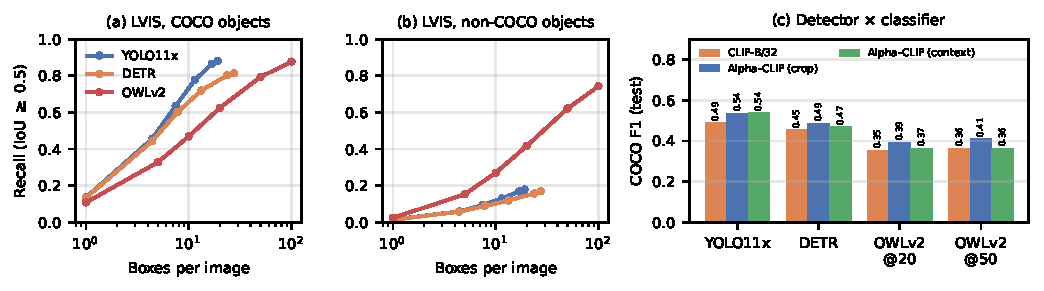
\includegraphics[width=\linewidth]{figures/fig_detector.pdf}
\caption{(a)(b) LVISの2148枚における1枚あたりのボックス数と検出の再現率（上位$ k $個のボックス，前稿の評価），(c) モデルの検出器と分類器を替えたテスト用の画像の$ F $（COCOの80クラスのF値）．}
\label{fig_detector}
\end{figure*}

図\ref{fig_detector}(a)(b)に，検出器の閾値を下げ，1枚あたり上位$ k $個のボックスを用いた場合の再現率を示す．
COCOの物体では，同じボックス数ならYOLO11xとDETRがOWLv2より高い．
YOLO11xとDETRは閾値を下げても約20〜30個でボックスが尽き，COCO外の物体の再現率は0.18以下にとどまった．
OWLv2は100個で0.743に達した．

\begin{table*}[t]
\vspace{4mm}
\centering
\caption{モデルの検出器を替えた比較（テスト用の画像，分類器はAlpha-CLIP（crop），残すボックスは式(\ref{eq_score})の規則）．記号は表\ref{tab_metrics}による（$ N $：残した数，Top-1：ラベルの正解率，$ P $：適合率，$ R $：再現率，$ F $：F値，$ hF $：細かい粒度の階層的F値，Acc：命名の正解率，Fine：正しくCOCOのクラスより細かい語を出力した割合，$ R_{\rm p} $：人物の再現率，$ R_{\rm N} $：残したボックスのCOCO外の物体の再現率）．}
\label{tab_pipeline}
\begin{tabular}{lrrrrrrrrrr}
\toprule
検出器 & $ N $ & Top-1 & $ P $ & $ R $ & $ F $ & $ hF $ & Acc & Fine & $ R_{\rm p} $ & $ R_{\rm N} $ \\
\midrule
YOLO11x（ボックスのみ） & 4.1 & 0.810 & {\bf 0.721} & 0.426 & {\bf 0.535} & 0.502 & 0.363 & 0.123 & 0.726 & 0.058 \\
DETR（ボックスのみ） & 5.3 & {\bf 0.819} & 0.562 & {\bf 0.428} & 0.486 & {\bf 0.521} & {\bf 0.385} & {\bf 0.136} & {\bf 0.739} & 0.061 \\
OWLv2（$ B = 20 $） & 4.4 & 0.777 & 0.507 & 0.322 & 0.394 & 0.428 & 0.235 & 0.104 & 0.421 & 0.094 \\
OWLv2（$ B = 50 $） & 5.3 & 0.796 & 0.472 & 0.363 & 0.411 & 0.461 & 0.274 & 0.111 & 0.545 & {\bf 0.103} \\
\midrule
Old（DETR＋CLIP） & 6.6 & 0.680 & 0.389 & 0.368 & 0.378 & 0.466 & 0.467 & 0.060 & 0.517 & -- \\
YOLO11x単体 & 5.7 & 0.976 & 0.796 & 0.655 & 0.719 & 0.670 & 0.816 & 0 & 0.766 & -- \\
\bottomrule
\end{tabular}
\end{table*}

表\ref{tab_pipeline}に，モデルの検出器を替えた検出から命名までの結果を示す．
$ F $はYOLO11xのボックスが0.535，DETRが0.486，OWLv2の$ B = 50 $が0.411であった．
OWLv2の$ B = 50 $との差は，YOLO11xが0.125（95\%区間［0.106，0.145］），DETRが0.075（［0.056，0.095］）であり，いずれも有意であった（$ p < 0.01 $）．
$ hF $もYOLO11xとDETRがOWLv2より0.04〜0.06高かった．
OWLv2の$ F $が低い主な原因は適合率$ P $であり，残したボックスのうちCOCOのGTに当たらないものが多い．
OWLv2の$ B = 50 $で残したボックスのうちCOCOのGTに当たらない41.3\%について，13.1\%はLVISのCOCO外の物体を囲んでいた（YOLO11xは7.0\%，DETRは3.4\%）．
LVISの注釈は網羅的でないため，この割合は下限である．
残したボックスのCOCO外の物体の再現率$ R_{\rm N} $は，OWLv2が0.103で最も高いものの，検出器の出力の0.734から大きく低下した．
$ \theta $をCOCOの80クラスの$ F $で選ぶため，COCO外の物体のボックスが残らないためである．
一方，COCOのクラスより細かい語を正しく出力した割合Fineは，いずれの検出器でも0.10〜0.14であり，Oldの0.060を上回った．
YOLO11x単体はCOCOの80クラスの$ F $が最も高いが，COCOのクラスより細かい語は出力できない．

\subsection{分類器の比較}
\begin{table}[t]
\centering
\caption{分類器の比較（テスト用の画像）．GTのボックスの列は検出の影響を除いた値であり，Top-1とTop-5はCOCOの80クラスの正解率，$ hF $は部分木の確率の合計による命名の階層的F値である（--：未評価）．右の4列は各検出器と組み合わせた場合の$ F $（COCOの80クラスのF値）である．}
\label{tab_classifier}
\setlength{\tabcolsep}{2.5pt}
\resizebox{\linewidth}{!}{%
\begin{tabular}{lrrrrrrr}
\toprule
 & \multicolumn{3}{c}{GTのボックス} & \multicolumn{4}{c}{$ F $（検出器と組み合わせ）} \\
分類器 & Top-1 & Top-5 & $ hF $ & YOLO & DETR & $ B {=} 20 $ & $ B {=} 50 $ \\
\midrule
CLIP（B/32） & 0.497 & 0.738 & 0.576 & 0.490 & 0.454 & 0.354 & 0.364 \\
Alpha-CLIP（crop） & {\bf 0.527} & 0.766 & -- & 0.535 & {\bf 0.486} & {\bf 0.394} & {\bf 0.411} \\
Alpha-CLIP（context） & {\bf 0.527} & {\bf 0.817} & {\bf 0.639} & {\bf 0.538} & 0.470 & 0.365 & 0.365 \\
\bottomrule
\end{tabular}}
\end{table}

表\ref{tab_classifier}に，分類器の比較を示す．
GTのボックスでは，Alpha-CLIPのTop-1は0.527であり，CLIPの0.497を上回った．
部分木の確率の合計による命名の$ hF $も，Alpha-CLIP（context）が0.639，CLIPが0.576であった（差0.063，［0.034，0.093］）．
検出器と組み合わせた場合，Alpha-CLIP（crop）の$ F $は，CLIPよりYOLO11xで0.045，DETRで0.032，OWLv2の$ B = 20 $で0.039，$ B = 50 $で0.047高く，いずれも有意であった（$ p \leq 0.001 $）．
Top-1も0.03〜0.07高かった．
一方，Alpha-CLIP（context）は，YOLO11xでは0.048高かったが，OWLv2ではCLIPとの差が有意でなかった．
contextの入力は周囲の領域を含むため，OWLv2の小さいボックスや物体の一部のボックスに周囲の物体の名前が付きやすい．
検出器と組み合わせた$ hF $の差は，いずれの組でも有意でなかった．
ただし，COCOのクラスより細かい語を正しく出力した割合Fineは，Alpha-CLIP（crop）が0.10〜0.14であり，CLIPの0.05〜0.06の約2倍であった．
命名の正解率AccはCLIPの方が0.12〜0.20高く，CLIPはpersonなどの粗い語を出力する割合が高い．
Alpha-CLIPは細かい語の確率を高く見積もるため，細かい語を出力する割合が増える一方，その一部は誤りとなる．
図\ref{fig_detector}(c)に，検出器と分類器の全ての組の$ F $を示す．

\subsection{語彙の木による粒度の判断}
本節では，検出の影響を除くため，GTのボックスに対して命名の手順を比較する．
VLMを用いない評価では，細かい正解のSynset自身がVGの語彙に含まれる割合は0.957であった．
語彙から1語を選ぶ場合の$ hR $の上限は，COCOの80クラスの0.597に対し，VGの語彙で0.990であった．

\begin{table}[t]
\centering
\caption{GTのボックスに対する命名の手順の比較（テスト用の画像）．$ hF $：細かい粒度の階層的F値，Acc：命名の正解率，Fine：正しくCOCOのクラスより細かい語を出力した割合．}
\label{tab_naming}
\setlength{\tabcolsep}{3pt}
\resizebox{\linewidth}{!}{%
\begin{tabular}{lrrrrrr}
\toprule
 & \multicolumn{3}{c}{CLIP（B/32）} & \multicolumn{3}{c}{Alpha-CLIP（context）} \\
命名の手順 & $ hF $ & Acc & Fine & $ hF $ & Acc & Fine \\
\midrule
COCOのクラスのみ & 0.373 & 0.518 & 0 & 0.266 & 0.307 & 0 \\
WordNetの下位語 & 0.373 & 0.503 & 0.029 & 0.266 & 0.304 & 0.015 \\
\rev{WordNet$ \cap $VGの木}の下位語 & 0.375 & 0.489 & 0.041 & 0.273 & 0.215 & 0.087 \\
VGの平坦な語彙 & 0.321 & 0.123 & 0.117 & 0.334 & 0.135 & 0.123 \\
部分木の合計 & 0.576 & 0.758 & 0.045 & {\bf 0.639} & {\bf 0.782} & 0.080 \\
\bottomrule
\end{tabular}}
\end{table}

表\ref{tab_naming}に結果を示す．
条件はいずれも検証用の画像の$ hF $で選んだ．
WordNetの下位語と\rev{WordNet$ \cap $VGの木}の下位語は，COCOのクラスから子のうち確率が最大の語を選んで下る手順である．
部分木の確率の合計は$ hF $を大きく高め，Alpha-CLIPではCOCOのクラスのみとWordNetの下位語の0.266から0.639に向上した．
VLMが人物の領域で持ち物の名前を最大にする場合でも，人物の部分木の確率が集まってpersonを出力できるためである．
部分木の確率の合計ではAlpha-CLIPがCLIPを上回ったのに対し，COCOのクラスのみでは下回った．
一方，COCOのクラスより細かい語を正しく出力できた割合は最大でも12.3\%であった．

\begin{figure}[t]
\centering
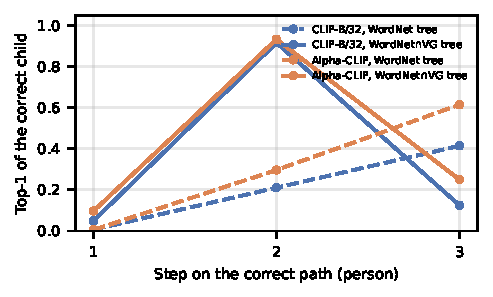
\includegraphics[width=0.95\linewidth]{figures/fig_step.pdf}
\caption{人物のGTのボックスで正しい経路を1段ずつ与えた場合の，各段の正しい子の選択の正解率（Top-1）．}
\label{fig_step}
\end{figure}

下位語をたどる手順が細かい語に届かない原因を調べるため，人物のGTのボックスで正しい経路を1段ずつ与え，各段で正しい子を選べる割合を求めた．
図\ref{fig_step}に結果を示す．
WordNetではpersonの直接の下位語が398語あり，1段目の正解率はAlpha-CLIPで0.005にとどまった．
\rev{WordNet$ \cap $VGの木}ではpersonの子が136語となり，1段目の正解率は0.097，2段目は0.933であった．

\subsection{定性評価}
図\ref{fig_qualitative}に，テスト用の画像に対する出力の例を示す．
(a)〜(c)では，部分木の確率の合計で選んだ語と，括弧内に深さ0のラベルを示す．
いずれの検出器でも，人物の領域にswimmer，surfer，tennis player，spectatorなどの細かい語が付き，同じ出力から深さ0のpersonも得られた．
YOLO11x単体はpersonのみを出力し，細かい語は出力できない．
OWLv2は波全体や画像全体などの大きな領域も囲み，surferのような場面の語を付けることがある．

\begin{figure*}[t]
\centering
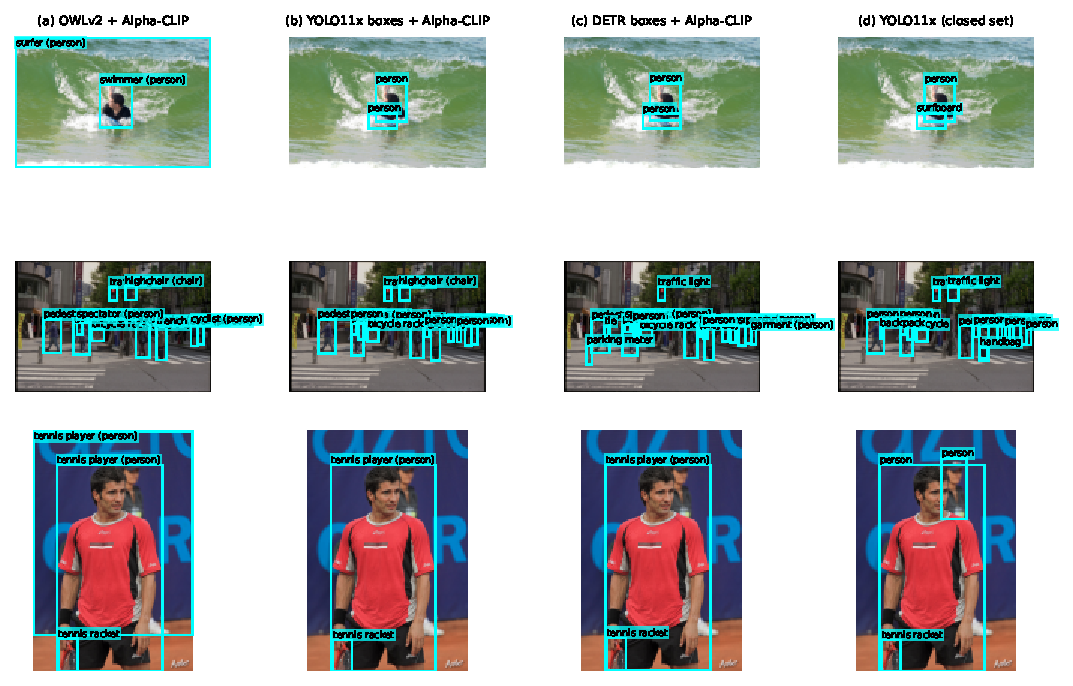
\includegraphics[width=0.82\linewidth]{figures/fig_qualitative.pdf}
\caption{テスト用の画像に対する出力の例．(a) OWLv2，(b) YOLO11xのボックス，(c) DETRのボックス（分類器はいずれもAlpha-CLIP（crop）），(d) YOLO11x単体．(a)〜(c)のラベルは式(\ref{eq_output})の出力であり，括弧内は深さ0のラベル$ c_k $である．}
\label{fig_qualitative}
\end{figure*}

\section{考察}
\subsection{検出器の選択}
検出の精度は，評価する物体によって順位が異なった．
COCOの物体に限れば，YOLO11xとDETRは少ないボックスで物体を囲み，GTに当たらないボックスも少ない．
そのため，COCOの80クラスで評価した検出から命名までの$ F $は，YOLO11xのボックスを用いた構成が最も高かった．
一方，COCO外の物体の再現率は，YOLO11xが0.100，DETRが0.124にとどまり，閾値を下げても0.18以下であった．
COCOで学習した検出器は，学習したクラスの物体以外を背景として扱うよう学習されているためである．

本稿の目的は，再学習なしに，COCOの80クラスより細かい語や80クラスの外の語で物体をアノテーションすることである．
検出器が囲まない物体は，分類器や語彙の木をどれだけ改善してもアノテーションできない．
したがって，検出器の再現率はアノテーションできる物体の上限を決める．
OWLv2の物体らしさは，学習時のクラスに依存せず，COCOの物体の87.5\%とCOCO外の物体の73.4\%を囲む唯一の検出器であった．
また，ボックス数$ B $により再現率を連続的に調整できる．
本稿でOWLv2を検出器に選ぶ理由はこの2点である．
YOLO11xやDETRを用いると，COCOの物体の$ F $は高まるが，COCO外の物体のアノテーションを諦めることになる．
なお，COCOの物体ではYOLO11xのボックスが有利であるため，YOLO11xのボックスとOWLv2のボックスを組み合わせることも有望である．

\subsection{分類器の選択}
Alpha-CLIPは，GTのボックスのTop-1と部分木の確率の合計による命名の$ hF $でCLIPを上回り，cropの入力では全ての検出器との組み合わせで$ F $がCLIPを上回った．
Alpha-CLIPは画像全体の文脈を保ったまま，αチャネルで指定した領域の特徴を求めるため，ボックスの内側だけを切り抜くCLIPより物体の識別に有利である．
また，COCOのクラスより細かい語を正しく出力した割合はCLIPの約2倍であり，粒度を変更するモデルの分類器として適している．
一方，命名の正解率はCLIPの方が高く，Alpha-CLIPは細かい語を出力する代わりに誤りも増える．
細かい語と正しさのどちらを優先するかは，式(\ref{eq_output})の閾値$ \tau $で調整できる．
contextの入力は周囲の物体の名前が付きやすく，ボックスの多いOWLv2との組み合わせではcropの入力が適していた．

\subsection{語彙の木による粒度の判断}
WordNetの下位語を1段ずつたどる命名では，personの直接の下位語が398語あり，1段目で正しい子を選べる割合は0.005にとどまった．
\rev{WordNet$ \cap $VGの木は，VGの注釈に現れる語のみで木を作るため，}personの子を136語に絞り，1段目の正解率を0.097に高めた．
さらに，部分木の確率の合計は，1段ずつの選択の誤りを積み重ねず，全ての語の確率から出力の深さを決める．
VLMの確率が人物の多くの下位語に分散する場合でも，部分木の合計はpersonのノードに集まるため，細かい語に確信が無ければpersonを出力する．
これが，GTのボックスで$ hF $が0.266から0.639に向上した理由である．
ただし，GTのボックスで正しくCOCOのクラスより細かい語を出力した割合は最大でも0.123であり，細かい粒度の命名の正しさには改善の余地がある．

\subsection{本稿の限界と今後の課題}
第一に，主な評価はCOCOの80クラスと，85\%が人物であるキャプションの細かい正解に基づく．
この評価はCOCOで学習した検出器に有利であり，COCO外の物体の命名の正しさは評価していない．
LVISのカテゴリはWordNetのSynsetを持つため，LVISの注釈を細かい正解とすれば，人物以外の物体で深さごとの命名を評価できる．
第二に，LVISの注釈は網羅的でなく，COCO外の物体の再現率と誤検出の内訳は概算である．
第三に，細かい正解はキャプションに基づくため，個々のインスタンスとは対応せず，第1語義の誤りを含む．
第四に，$ B = 50 $のOWLv2の推論のため，処理時間はOldの約5倍である．
第五に，残すボックスを決める規則は，COCOの80クラスの部分木の確率の合計と物体らしさの積を用い，$ \theta $をCOCOの$ F $で選ぶため，COCO外の物体のボックスは残らない．
その結果，検出器の出力では0.734であったCOCO外の物体の再現率が，残したボックスでは0.103に低下した．
COCO外の物体を残す棄却のスコアの設計と，その評価は今後の課題である．

\section{おわりに}
本稿では，OWLv2の物体らしさ，Alpha-CLIP，\rev{WordNetとVGを組み合わせた語彙の木}を組み合わせ，再学習を必要とせずにカテゴリの粒度を変更できる物体アノテーションのモデルを示し，検出器と分類器を選ぶ理由を実験により示した．
COCO 2017 Validationの評価では，OWLv2の物体らしさは1枚あたり50個のボックスでCOCOの物体の87.5\%とCOCO外の物体の73.4\%を囲み，COCO外の物体の再現率が0.1程度にとどまるYOLO11xとDETRに対して，アノテーションできる物体の範囲が広いことを示した．
一方，COCOの80クラスによる$ F $は，YOLO11xのボックスを用いた構成が0.535，DETRが0.486，OWLv2が0.411であり，COCOの物体に限ればCOCOで学習した検出器が有利であった．
分類器は，全ての検出器でAlpha-CLIP（crop）がCLIPより$ F $を0.03〜0.05高め，COCOのクラスより細かい語を正しく出力した割合をCLIPの約2倍とした．
また，語彙の木の部分木ごとに確率を合計して出力の深さを決めることで，GTのボックスの階層的F値がCOCOのクラスのみの0.266から0.639に向上した．
今後の課題として，COCO外の物体を残す棄却のスコアの設計，LVISの注釈による人物以外の物体の粒度の評価，YOLO11xとOWLv2のボックスの組み合わせ，処理時間の短縮が挙げられる．

\vspace{-1mm}
\begin{thebibliography}{99}
\small

    \bibitem{ref_YOLO}
    J. Redmon, S. Divvala, R. Girshick, and A. Farhadi,
    ``You Only Look Once: Unified, Real-Time Object Detection,''
    in {\it Proc. IEEE Conference on Computer Vision and Pattern Recognition (CVPR)}, 2016.

    \bibitem{ref_DETR}
    N. Carion, F. Massa, G. Synnaeve, N. Usunier, A. Kirillov, and S. Zagoruyko,
    ``End-to-End Object Detection with Transformers,''
    in {\it Proc. European Conference on Computer Vision (ECCV)}, 2020.

    \bibitem{ref_COCO}
    T.-Y. Lin, M. Maire, S. Belongie, J. Hays, P. Perona, D. Ramanan, P. Doll\'{a}r, and C. L. Zitnick,
    ``Microsoft COCO: Common Objects in Context,''
    in {\it Proc. European Conference on Computer Vision (ECCV)}, pp. 740--755, 2014.

    \bibitem{ref_prev}
    著者名,
    ``物体領域検出とカテゴリアノテーションの分離に基づく，WordNetを用いた粒度可変物体アノテーション,''
    2026.

    \bibitem{ref_prevVG}
    著者名,
    ``人の命名の頻度に基づく語彙と確率の集約による粒度可変な物体アノテーションの改善,''
    2026.

    \bibitem{ref_WordNet}
    G. A. Miller,
    ``WordNet: A Lexical Database for English,''
    {\it Communications of the ACM}, vol. 38, no. 11, pp. 39--41, 1995.

    \bibitem{ref_CLIP}
    A. Radford, J. W. Kim, C. Hallacy, A. Ramesh, G. Goh, S. Agarwal, G. Sastry, A. Askell, P. Mishkin, J. Clark, G. Krueger, and I. Sutskever,
    ``Learning Transferable Visual Models From Natural Language Supervision,''
    in {\it Proc. International Conference on Machine Learning (ICML)}, 2021.

    \bibitem{ref_OWLv2}
    M. Minderer, A. Gritsenko, and N. Houlsby,
    ``Scaling Open-Vocabulary Object Detection,''
    in {\it Proc. Advances in Neural Information Processing Systems (NeurIPS)}, 2023.

    \bibitem{ref_AlphaCLIP}
    Z. Sun, Y. Fang, T. Wu, P. Zhang, Y. Zang, S. Kong, Y. Xiong, D. Lin, and J. Wang,
    ``Alpha-CLIP: A CLIP Model Focusing on Wherever You Want,''
    in {\it Proc. IEEE/CVF Conference on Computer Vision and Pattern Recognition (CVPR)}, 2024.

    \bibitem{ref_VG}
    R. Krishna, Y. Zhu, O. Groth, J. Johnson, K. Hata, J. Kravitz, S. Chen, Y. Kalantidis, L.-J. Li, D. A. Shamma, M. S. Bernstein, and L. Fei-Fei,
    ``Visual Genome: Connecting Language and Vision Using Crowdsourced Dense Image Annotations,''
    {\it International Journal of Computer Vision}, vol. 123, pp. 32--73, 2017.

    \bibitem{ref_OWLViT}
    M. Minderer, A. Gritsenko, A. Stone, M. Neumann, D. Weissenborn, A. Dosovitskiy, A. Mahendran, A. Arnab, M. Dehghani, Z. Shen, X. Wang, X. Zhai, T. Kipf, and N. Houlsby,
    ``Simple Open-Vocabulary Object Detection with Vision Transformers,''
    in {\it Proc. European Conference on Computer Vision (ECCV)}, 2022.

    \bibitem{ref_CHiLS}
    Z. Novack, J. McAuley, Z. C. Lipton, and S. Garg,
    ``CHiLS: Zero-Shot Image Classification with Hierarchical Label Sets,''
    in {\it Proc. International Conference on Machine Learning (ICML)}, 2023.

    \bibitem{ref_hier}
    S. Kiritchenko, S. Matwin, R. Nock, and A. F. Famili,
    ``Learning and Evaluation in the Presence of Class Hierarchies: Application to Text Categorization,''
    in {\it Proc. Canadian Conference on Artificial Intelligence}, pp. 395--406, 2006.

    \bibitem{ref_YOLO11}
    G. Jocher and J. Qiu,
    ``Ultralytics YOLO11,''
    \url{https://github.com/ultralytics/ultralytics}, 2024.

    \bibitem{ref_LVIS}
    A. Gupta, P. Doll\'{a}r, and R. Girshick,
    ``LVIS: A Dataset for Large Vocabulary Instance Segmentation,''
    in {\it Proc. IEEE/CVF Conference on Computer Vision and Pattern Recognition (CVPR)}, 2019.

\end{thebibliography}


\end{document}
